\chapter{Combinatorics}
Combinatorics is one of the most fascinating and frustrating branches of mathematics. Many excellent mathematics students find it impossibly difficult while some find it as easy as breathing. Classically, combinatorics deals with finite sets of objects and the various ways their subsets and their elements can be counted and ordered.

One of the first formal attempts of combinatorial thinking seems to have come around $960$, when \index{Bishop Wibold of Cambrai} correctly enumerated the $56$ outcomes that can arise when three dice are thrown simultaneously: $\{1, 1, 1; 1, 1, 2; 1, 1, 3, ...\}$ and so on. A thirteenth-century Latin poem, \index{DeVetula}, listed the $216 (= 6 \cdot 6 \cdot 6)$ outcomes that may result when three dice are thrown in succession. 

If the results $56$ and $216$ seams somewhat unclear, don't dispair this chapter will teach you how to arrive at these results safely on your own.

 % TODO explain why the first is 56 and the second 216

So, in Mathematics we use more precise language:

	If the order doesn't matter, it is a Combination.
	If the order does matter it is a Permutation.

A Permutation is an ordered Combination.

\section{Permutations}
In other words:

You've decided to take $3$ steps and randomly choose left or right as the direction each time. How many different outcomes exists?. The mathematical branch of combinatorics helps us answers questions such as these and its mastery is essential to study statistics. Returning to our example we notice that you have two possibilities for the first step, two possibilities for the second and again two possibilities for the third yielding $2 \cdot 2 \cdot 2 = 8$. The figure below shows the situation:
\begin{figure}[H]
\centering
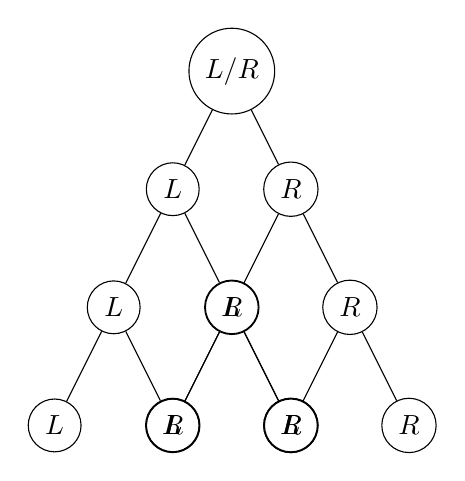
\begin{tikzpicture}
\node[circle,draw](1){$L/R$}
  child {
      node [circle,draw](2){$L$}
         child {
             node [circle,draw](3){$L$}
                   child { node [circle,draw](4){$L$}}
                   child { node [circle,draw](5){$R$}}
         }
         child {
             node [circle,draw](6){$R$}
                   child { node [circle,draw](7){$L$}}
                   child { node [circle,draw](8){$R$}}
         }
   }
   child {
       node [circle,draw](9){$R$}
         child {
             node [circle,draw](10){$L$}
                   child { node [circle,draw](11){$L$}}
                   child { node [circle,draw](12){$R$}}
         }
         child {
             node [circle,draw](13){$R$}
                   child { node [circle,draw](14){$L$}}
                   child { node [circle,draw](15){$R$}}
         }
   };
\end{tikzpicture}
\end{figure}

Suppose we have before us 2 red aces and 2 red kings from the usual deck of 52 cards. How many different pairs consisting of one ace and one king can be put together? Since each ace can be paired with either of 2 kings, there are 2 different pairs for any one ace. Since we have 2 aces, there are $2 \cdot 2$ or 4 different pairs.

\section{Counting selections}
Consider in how many ways can we arrange the set $\{1,2,3\}$:
\[
\{1, 2, 3\}, \{1, 3, 2\}, \{2, 1, 3\}, \{2, 3, 1\}, \{3, 1, 2\}, \{3, 2, 1\}
\]
that is we have $3$ ways of choosing the first element, and $3-1$ options for the second (as we cannot repeat the first choise) and $3-2$ for the last (as non of the former two choices may be used), therefor we can arrange them in $3 \cdot 2 \cdot 1 = 6$ ways. In general we define the number of permutations of a set with $n$ elements as the faculty function $n!$
\[
n! = n \cdot (n-1) \cdot (n-2) \cdots  (n - (n -1)) = 1 \cdot 2 \cdots n = \prod_{k=1}^{n}k,
\]

the last notation simply means that we multiply all the values of $k$ from $1$ to $n$. A recursive version (a self-calling function) can be constructed by noting that $n! = n(n-1)!$. \\

\myindent Now consider a slightly more complex question: in how many ways can we pick two elements from the set $\{1,2,3\}$, the answer turns out to be three ways:
\[
\{1, 2\}, \{1, 3\}, \{2, 3\}
\]
To generalize this we can ask in how many ways can we pick a unordered subset with $k$ elements from a set with $n$ elements ?. To answer this, observe there are $n$ choices for the first element and for each of these there are $n - 1$ choices for the second; and so on until there are $n - k + 1$ for the k'th element. That is we have $n \cdot (n-1) \cdots (n - k + 1)$ ways for picking a $k$-element subset from $n$. As we are picking unordered sets and since each $k$-element subset has exactly $k!$ different orderings, we get our answer by dividing with $k!$:
\begin{equation}\label{binom}
\binom{n}{k} = \frac{n(n-1) \cdots (n - k + 1)}{k!},  \qquad \text{integer } n \geq k \geq 0
\end{equation}
and if we multiply the numerator and denominator of \ref{binom} by $(n - k)!$ we get:
\[
\frac{n(n-1) \cdots (n - k + 1)}{k!} \cdot \frac{(n - k)!}{(n - k)!} =  \frac{n!}{k!(n-k)!}
\]
The symbol $\binom{n}{k}$ is known as a binomial coefficient and we read it "$n$ choose $k$" (the number of ways to select $k$ elements from $n$ element set). Using this result we can directly answer the above question of how many ways to choose two elements from a three element set:
\[
\binom{3}{2}  = \frac{3!}{2! (3-2)!} = \frac{3 \cdot 2 \cdot 1}{2 \cdot 1 \cdot 1} = 3
\]
Interestingly when determining the number of ways to pick $k$ elements we have in effect also specified the $n-k$ unchosen things, therefore
\begin{equation}\label{binom_symmetry}
\binom{n}{k} = \binom{n}{n-k}
\end{equation}
this symmetry can be observed in the above example where we have $3$ ways of picking $2$ elements from a $3$-element set but then also $3$ ways of picking the remaining element. It also follows directly from the definition of the binomial coefficient
\[
\binom{n}{k} =  \frac{n!}{k!(n-k)!} =  \frac{n!}{(n-(n-k))!(n-k)!} = \binom{n}{n-k}
\]

\myindent Another rather remarkable result, known as Pascal's rule, can be derived by marking a particular object $\epsilon$ in an $n$-element set. Now if we pick $k$ objects from $n$, then either $\epsilon$ is picked or it is not. If $\epsilon$ is in the subset then there is $k-1$ objects left to choose among the $n-1$ elements, or more formally $\binom{n-1}{k-1}$. If $\epsilon$ is not in the subset, we need to choose all the $k$ elements in the subset from the $n-1$ objects that are not $\epsilon$; formally that is $\binom{n-1}{k}$. Thus there are
\[
\binom{n-1}{k-1} + \binom{n-1}{k}
\]
ways to choose $k$ elements from $n$ depending on whether $\epsilon$ is included in each selection or not. But this number must be the same as the binomial coefficient and thus we get:
\begin{equation}\label{pascal_rule}
\binom{n}{k}  = \binom{n-1}{k-1} + \binom{n-1}{k}
\end{equation}
this result can also be arrived at by algebraic manipulation
\begin{align*}
 \binom{n-1}{k-1} + \binom{n-1}{k}
& =  \frac{(n-1)!}{(k-1)!((n-1)-(k-1))!} + \frac{(n-1)!}{k!((n - 1) - k)!} \\
& =  \frac{(n-1)!}{(k-1)!(n-k)!} + \frac{(n-1)!}{k!(n - (k + 1))!} \\
& =  \frac{k(n-1)!}{k!(n-k)!} + \frac{(n-1)!(n-k)}{k!(n - k)!} \\
& =  \frac{(n-1)!(k + n - k)}{k!(n-k)!} \\
& =  \frac{n!}{k!(n-k)!}
\end{align*}

%% PASCALs TRIANGLE
\myindent From Pascal's rule we can construct his famous triangle. Observe that according to this rule (see \ref{pascal_rule}) you can calculate $\binom{5}{3}$ as:
\begin{align*}
 \binom{5}{3}
& =  \binom{4}{3} + \binom{4}{2}  \\
& =  \binom{4}{3} + \binom{3}{2} +  \binom{3}{1} \\
& =  \binom{4}{3} + \binom{3}{2} +  \binom{2}{1} + \binom{2}{0} \\
\end{align*}
as $\binom{2}{0} = 1$, we can stop the expansion. In general as $\binom{n}{n}$ and $\binom{n}{0}$ are always $1$ (when $n \geq 0$) we are guarantied that the expansion always terminates. Thus we have found a convenient way of expressing higher binomial coefficients as sums of consecutive smaller ones:
\begin{center}
\begin{tabular}{l|*{5}{c}r}
\toprule
$n$ & $\binom{n}{0}$        & $\binom{n}{1}$ & $\binom{n}{2}$ & $\binom{n}{3}$ & $\binom{n}{4}$  & $\binom{n}{5}$ \\
\hline
0		& 1                     & 0 			       & 0 			        & 0 			       & 0 			         & 0   \\
1   & 1                     & 1 			       & 0 			        & 0 			       & 0  			       & 0   \\
2   & 1                     & 2 			       & 1 			        & 0 			       & 0  			       & 0   \\
3		& 1                     & 3 			       & 3 			        & 1			         & 0  			       & 0   \\
4		& 1                     & 4 			       & 6 			        & 4			         & 1  			       & 0   \\
5		& 1                     & 5 			       & 10 			      & 10			       & 5  			       & 1   \\
\bottomrule
\end{tabular}
\end{center}
discarding the zero's we can arrange these numbers into a triangle:
\[
\begin{array}{c}
1 \\
1\ \myindent 1\\
1\ \myindent 2\ \myindent 1   \\
1\ \myindent 3\ \myindent 3\   \myindent 1   \\
1\ \myindent 4\ \myindent 6\   \myindent 4\   \myindent 1\\
1\ \myindent 5\ \myindent 10\ \myindent 10\ \myindent 5\ \myindent1\\
\ \textnormal{and so on} \ \\
\end{array}
\]
where the next row must contain:
\[
\binom{6}{0} \myindent \binom{6}{1} \myindent \binom{6}{2} \myindent \binom{6}{3} \myindent \binom{6}{4} \myindent \binom{6}{5} \myindent \binom{6}{6}
\]
but we already know that expressions like $\binom{6}{1}$ can be rewritten to
$\binom{5}{1} + \binom{5}{0} = 5 + 1$. So we see that each entry in the new row
is obtained simply by adding the numbers in the row above to the left and right.
\[
1\ \myindent 6\ \myindent 15\ \myindent 20\ \myindent 15\ \myindent 6\ \myindent 1
\]

To generate the triangle, you start with a 1, and then immediately below it, you put two 1’s, one to either side. Then for each successive row, you put a new 1 at either end and complete the row between them by adding together each adjacent pair of entries in the row above and putting their sum halfway between them.

% TODO binomials (a+b)^2 = 1 2 1, (a+b)^3 = 1 3 3 1

\newpage
%%
\section{Newton's Binomial Theorem}
In mathematics a binomial is a polynomial with two terms, i.e such as these
\[\begin{array}{lcl}
(a + b)^0 &=& 1\\
(a + b)^1 &=& a + b \\
(a + b)^2 &=& a^2 + 2ab + b^2 \\
(a + b)^3 &=& a^3 + 3a^2b + 3ab^2 + b^3 \\
(a + b)^4 &=& a^4 + 4a^3b + 6a^2b^2 + 4ab^3 + b^4 \\
:                &   & :
\end{array}\]
or in general
\[
(a+b)^n = \overbrace{(a+b)(a+b)\cdots(a+b)}^{n\textnormal{ factors}}
\]
the relationship between such polynomials and combinatorics stems from the so called binomial theorem.

%\newpage
%\section*{Exercises}
%\addcontentsline{toc}{section}{Exercises}
%\subsection*{Warmups}
% 1
%\begin{exc}\label{ex:analysis:1}
%Show that
%\[
%\binom{n}{0} + \binom{n}{1} + \cdots + \binom{n}{n - 1} + \binom{n}{n} = 2^n
%\]
%\end{exc}
% 2

\section{Exercises}
\begin{ExerciseList}

\Exercise Count the following
\Question A gardening store offers $4 $ different flowers and $4$ different types of pots how many different arrangement of pot and plant can you make
\Question A girl has $3$ hats, $2$ dresses, and $2$ pairs of shoes. How many different costumes does she have?
\Question A deck of $52$ cards contains $4$ different aces and $4$ different kings. How many different pairs of cards, each pair consisting of one ace and one king, can be formed from the aces and kings?
\Question In how many different ways can $7$ people sit in $3$ chairs ?
\Question There are $7$ people in a room. If everyone shakes everyone else's hand exactly once, how many handshakes occur? 
\Answer Using the rules of counting we find
\begin{enumerate}
\item \myindent Each of the four plants can be placed in four different pots yielding $4 \cdot 4 = 16$ possible arrangements
\item \myindent TODO describe why $3 \cdot 2 \cdot 2 = 12$
\item \myindent TODO describe why $4 \cdot 4$
\item \myindent $7$ different ways to pick the first chair, leaving $6$ different people to pick the second chair, leaving $5$ different people to pick the fifth chair i.e. $7*6*5 = 210$
\item \myindent $\frac{7*6}{2}$ handshakes will occur as each of the seven people will shake hands with six other people but since one person shaking with another is counted twice we divide with two.
\end{enumerate}

\end{ExerciseList}

